\subsection{Überblick}
\pgfdeclarelayer{background}
\pgfsetlayers{background,main}

\tikzstyle{vertex}=[circle,fill=black!25,minimum size=20pt,inner sep=0pt]
\tikzstyle{selected vertex} = [vertex, fill=red!24]
\tikzstyle{blue vertex} = [vertex, fill=blue!24]
\tikzstyle{edge} = [draw,thick,-]
\tikzstyle{weight} = [font=\small]
\tikzstyle{selected edge} = [draw,line width=5pt,-,red!50]
\tikzstyle{ignored edge} = [draw,line width=5pt,-,black!20]

\begin{frame}{Random Walk}
    \begin{figure}
        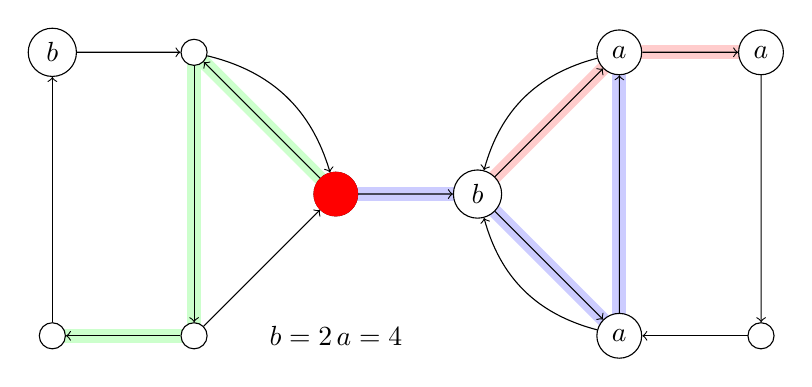
\begin{tikzpicture}[->,scale=1.8, auto,swap]
            % Draw the vertices. First you define a list.
            \foreach \pos/\name/\ltext in {{(0,0)/a/}, {(0,2)/b/b}, {(1,2)/c/},
                                    {(1,0)/d/}, {(2,1)/e/e}, {(3,1)/f/b}, 
                                    {(4,2)/g/a}, {(5,2)/h/a}, {(4,0)/i/a},
                                    {(5,0)/j/}}
                \node[draw,circle,fill=white] (\name) at \pos {$\ltext$};

            \node[draw,circle,red,fill=red] (e) at (2,1) {$e$};

            % Connect vertices with edges and draw weights
            \foreach \source/ \dest /\pos in {a/b/, b/c/, c/d/, d/a/,
                                        c/e/bend left, d/e/, e/c/,
                                        e/f/, f/g/, f/i/,
                                        g/f/bend right, i/f/bend left,
                                        g/h/, h/j/, j/i/, i/g/}
                \path (\source) edge [\pos] node {} (\dest);

            \foreach \fr / \number in {1/,
                2/b=1,
                3/b=1\, a=1,
                4/b=1\, a=2,
                5/b=2\, a=2,
                6/b=2\, a=3,
                7/b=2\, a=4
                }
                \node<\fr->[fill=white] (Tlabel) at (2,0) {$\number$};

            % Start animating the edge selection. 
            % For convenience we use a background layer to 
            % highlight edges. This way we don't have to worry about 
            % the highlighting covering weight labels. 
            \begin{pgfonlayer}{background}
                \foreach \source / \dest / \fr / \colorf /\pos in {e/f/2/red/,f/g/3/red/,g/h/4/red/, e/f/5/blue/, f/i/6/blue/, i/g/7/blue/,e/c/8/green/,c/d/9/green/, d/a/10/green/}
                    \path<\fr->[selected edge, \colorf!20] (\source.center) edge 
                                        [\pos] node {} (\dest.center);
            \end{pgfonlayer}
        \end{tikzpicture}
    \end{figure}

    Klassifizieren des roten Knotens:
    \begin{itemize}
        \item Zählen von Knotenbeschriftungen in Random Walks
        \item 4 Random Walks
        \item 3 Sprünge pro Random Walk
        \item<11> $4 \cdot a$, $2 \cdot b \Rightarrow$ Rot mit $a$ klassifizieren
    \end{itemize}
\end{frame}

\begin{frame}{Wortknoten}
    \begin{itemize}
        \item<1-> Neben Struktur können Texte genutzt werden
        \item<2-> Einschränkung: Effizienz!
        \item<3-> Wünschenswert: Wenig weiterer Programmieraufwand
        \item<4-> Idee: Graph erweitern
        \begin{itemize}
            \item<5-> Texte als Wortmengen
            \item<6-> Strukturknoten verweisen auf Wortknoten
            \item<7-> vice versa
        \end{itemize}
    \end{itemize}
\end{frame}

\framedgraphic{Erweiterter, bipartiter Graph}{../images/graph-content-and-structure.pdf}
